% This is LLNCS.DEM the demonstration file of
% the LaTeX macro package from Springer-Verlag
% for Lecture Notes in Computer Science,
% version 2.4 for LaTeX2e as of 16. April 2010
%
\documentclass{llncs}
%
\usepackage{makeidx}  % allows for indexgeneration
\usepackage[pdftex]{graphicx}
\usepackage[T1]{fontenc}
\usepackage[utf8]{inputenc}
\usepackage{upquote}
%
\begin{document}
%
\mainmatter              % start of the contributions
%
\title{A text model - Use your favourite M2M for M2T}
%
\titlerunning{Textual M2M}  % abbreviated title (for running head)
%                                     also used for the TOC unless
%                                     \toctitle is used
%
\author{Edward D. Willink}
%
\authorrunning{Edward Willink} % abbreviated author list (for running head)
%
%%%% list of authors for the TOC (use if author list has to be modified)
\tocauthor{Edward Willink}
%
\institute{Willink Transformations Ltd, Reading, England,\\
\email{ed\_at\_willink.me.uk}}


\maketitle              % typeset the title of the contribution

\begin{abstract}
Models provide a disciplined representation of information. Model-to-Model (M2M) transformations convert between model structures. When a more readable representation is required, Model-to-Text (M2T) transformations convert a model structure to a concatenation of character sequences. We ignore the obvious conversion differences and demonstrate that an unmodified M2M tool can be used for M2T. We achieve this with a standard Text model that post-processes the M2M model output to yield formatted text. 

\keywords{Model transformation, M2M, M2T, Text model}
\end{abstract}
%
\section{Introduction}
%
For model enthusiasts, everything is a model and every change is a model-to-model transformation. Models are persisted in a form that is suitable for automated use, often involving XMI files or model databases. Unfortunately, in the real world there are many occasions where a practical representation of a model is required. If the information is to be maintained by humans, something more readable than XML is required. If the information is to be consumed by a tool, such as a C compiler that has no knowledge of models, the information must be provided in the tool-specific language, such as C. A model-to-text transformation is therefore required to provide the model in the required form.

An M2T destroys models whereas an M2M preserves models; consequently there is an orthodoxy that M2M and M2T are different technologies. An M2T language is designed around string template expressions, whereas an M2M language is designed around model mappings. This orthodoxy is endorsed by the Object Management Group (OMG) where M2M is facilitated by the Query/View/Transformation (QVT) specification \cite{QVT-1.3} and M2T by the MOFM2T specification \cite{MOFM2T-1.0}. There are a variety of correspondingly named implementations of the QVT languages \cite{Eclipse-QVTd}, \cite{Eclipse-QVTo}. Acceleo \cite{Eclipse-Acceleo} is the only (partial) implementation of MOFM2T.

In this paper we examine the distinctive characteristics of M2T in Section~\ref{M2T} before examining an M2M solution in Section~\ref{M2M}. In Section~\ref{Evaluation} we evaluate the solution before outlining future work in Section~\ref{Future Work}. We consider related work in Section~\ref{Related Work} and conclude in Section~\ref{Conclusions}. 

\section{Is M2T necessarily distinct?}\label{M2T}

At this point I must thank Toni Siljamaki for his obstinate persistence in asking why Eclipse QVTo couldn't be used to perform M2T \cite{Bug396543}. My initial instinctive reaction was to fall back on orthodoxy; OMG provide distinct specifications and anyway M2M and M2T are obviously different. However after some reflection, it is clear that the "M2" facilities such as metamodels, loading, navigation, expressions, queries and rules are the same for both M2M and M2T. Only the final "2M" or "2T" need be different. Requiring the use of distinct M2M and M2T tools is not justifiable.

How might an M2M support text? Only one change and one enhancement appear to be necessary:

\begin{itemize}
	\item change: output to a text file rather than model file
	\item enhancement: better facilities for creating strings / character sequences
\end{itemize}

\subsection{Text Output}\label{Text Output}

In MOFM2T, the rules (templates) conspire to concatenate and return Strings. M2M tools can already do this since the underlying language, typically OCL \cite{OCL-2.4}, has a String type and String operations. It is just necessary to amend the output model declaration to identify that the overall String result is to be emitted directly as a text File, rather than encoded as an XML file.

\subsection{Text Facilities}\label{Text Facilities}

Considering the following example output text:

\begin{verbatim}
The name is "computedName".
\end{verbatim}

Typical M2T tools such as Acceleo or Xtend provide a forward escape to embed a control expression within literal text. 

\begin{verbatim}
The name is "[self.name/]".  -- MOFM2T/Acceleo with escaped OCL
The name is "«this.name»".   -- Xtend with escaped Java
\end{verbatim}

A backwards escape may define a multi-line text expression that concatenates with its siblings and may have nested forward escapes. However an OCL-based M2M without escapes may only concatenate explicitly.

\begin{verbatim}
'The name is "[self.name/]".'       -- MOFM2T
'''The name is "«this.name»".'''    -- Xtend
\end{verbatim}

An OCL-based M2M without escapes may only concatenate explicitly.

\begin{verbatim}
'The name is "'+ self.name +'".'    -- OCL
\end{verbatim}

OCL provides a fairly modest String library and an overall expression evaluation capability that allows complex String results to be computed. No change is therefore mandated to enable an OCL-based M2M to be used as an M2T although enhanced String capabilities could well be helpful for applications with a high proportion of literal text.

Considering the following example output with a repeated computation:

\begin{verbatim}
{ "firstComputedName", "secondComputedName" }
\end{verbatim}

A for loop facility with optional before/prefix, separator and after/suffix texts is helpful. The examples below show Acceleo and then Xtend.

\begin{verbatim}
{ [for (p : P | somePs) separator(', ')]"[p.name/]"[/for] }
{ «FOR p : somePs SEPARATOR ', '»"«p.name»"«ENDFOR» } 
\end{verbatim}

An OCL-based M2M may use collect() for the content iteration, but the separator splicing is verbose.

\begin{verbatim}
'{ '+ somePs->collect(p | '"'+ p.name +'"')
  ->iterate(s; acc : String = '' |
      if acc = '' then s else acc +', '+ s endif
    )  +' }'
\end{verbatim}

\section{M2M solution}\label{M2M}

Figure~\ref{fig:ModelM2M} shows the typical components of an M2M transformation and associated environment that we re-use for M2T. The core M2M transforms between input and output models, each of which conforms to its corresponding metamodel, which in turn conforms to a universal metametamodel such as Ecore. The input model is loaded from an input file by an XMI load facility, and the output model is saved by a corresponding XMI save facility.

\begin{figure}
	\begin{center}
		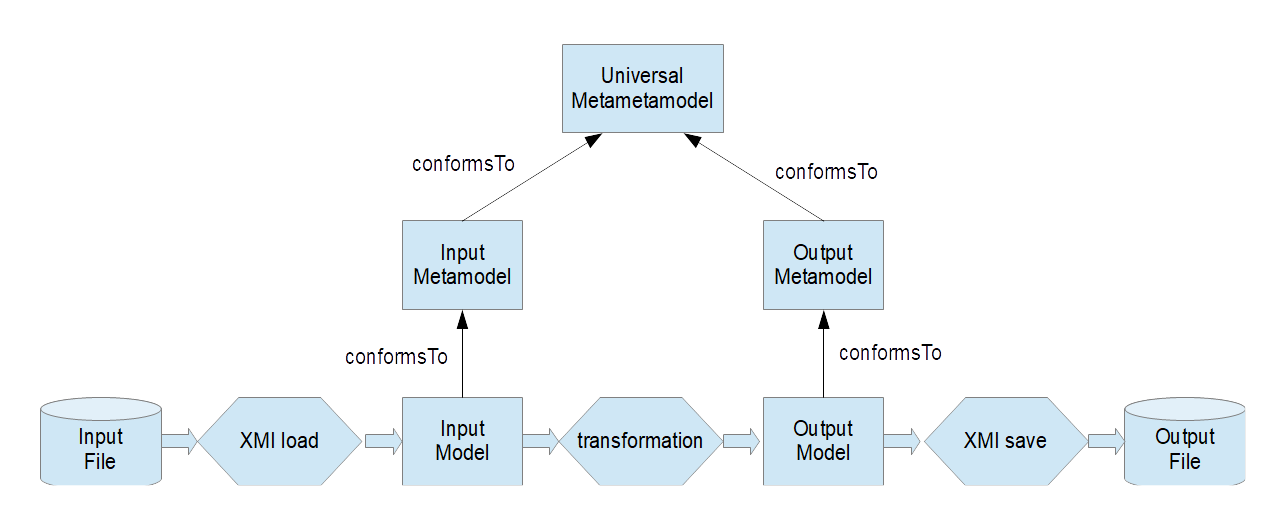
\includegraphics[width=4.9in]{ModelM2M.png}
	\end{center}
	\caption{M2M for models}
	\label{fig:ModelM2M}
\end{figure}

After many years reflection, the solution to using an M2M for M2T arose from another longstanding problem; how can an M2M be used to perform an XML2XML transformation?

\subsection{XML2XML}\label{XML2XML}

The need for an XML2XML transformation arises when there is a need to manipulate some aspect of the XMI serialization of a model in a way that is not accessible to a regular M2M. Typically there may be a need to impose some policy on the xmi:ids that are a serialization rather than model artefact. There is no xmi:id within the model technology space and so any solution that tries to expose an xmi:id is messy.

\begin{figure}
	\begin{center}
		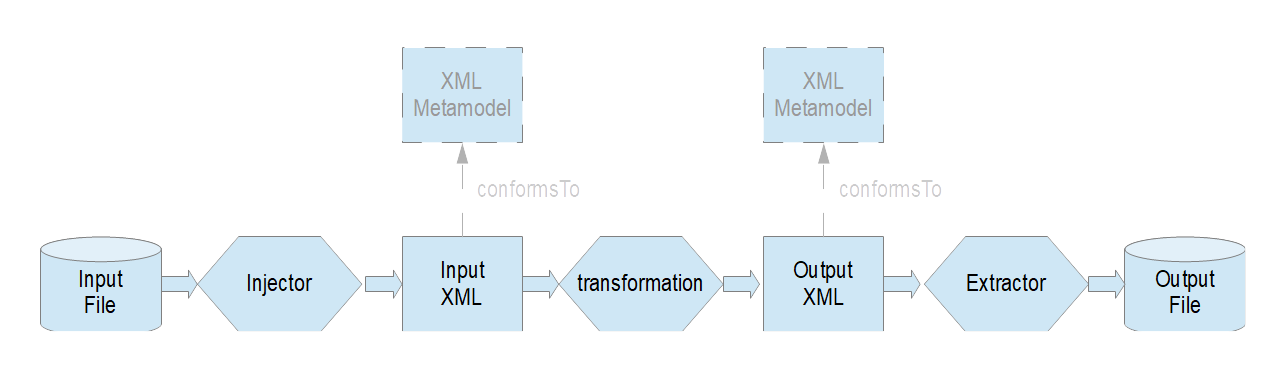
\includegraphics[width=4.9in]{ATLXMLM2M.png}
	\end{center}
	\caption{ATL injector and extractor for XML M2M}
	\label{fig:ATLXMLM2M}
\end{figure}

B\'ezevin \cite{TechnologySpace} identified distinct model, grammar and XSD technology spaces and the early versions of ATL \cite{Eclipse-ATL} supported XML2XML transformation through the use of custom injectors and extractors as shown in Figure~\ref{fig:ATLXMLM2M}. ATL's weak metamodel typing allowed the XML metamodel to remain a little vague. Unfortunately these custom load and save functionalities have suffered from bit rot and are no longer available; XML2XML is no longer supported by ATL. 

%If however a transformation is performed in the XML technology space, the xmi:id is there and can be manipulated as desired. Of course we do not want to have to use separate XML and Model technology space transformation tools, and so since XML is self-evidently a model, how can an M2M be used for XML2XML? The original implementation of the ATL M2M that accompanied the technology space papers provided alternative 'injectors' so that a model could be loaded in its XML-conforming rather than Ecore-conforming form.

\begin{figure}
	\begin{center}
		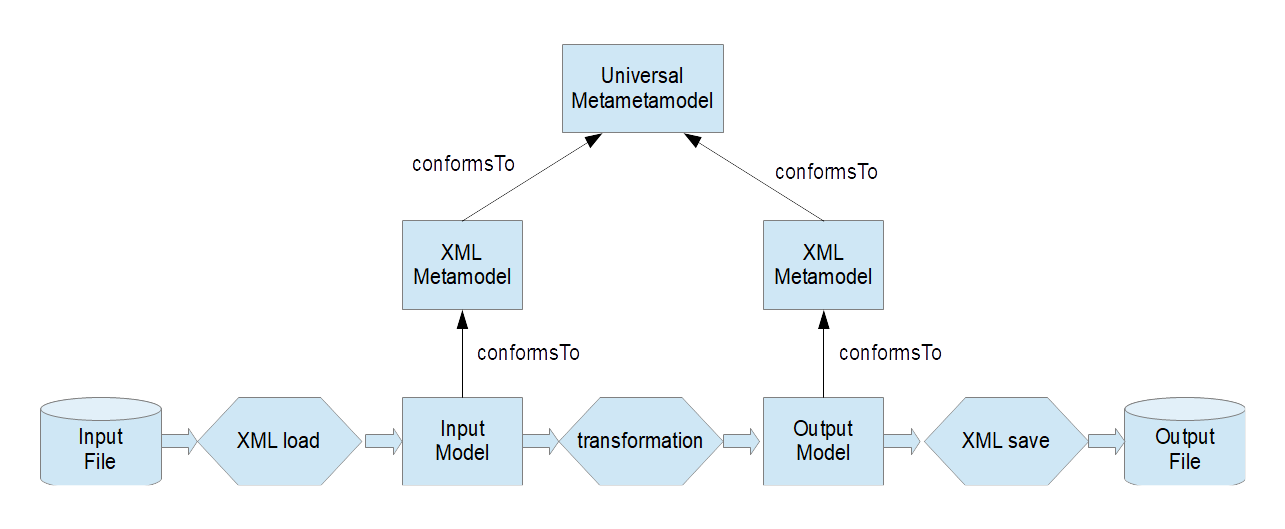
\includegraphics[width=4.9in]{XMLM2M.png}
	\end{center}
	\caption{Variant EMF loader and saver for XML Model M2M}
	\label{fig:XMLM2M}
\end{figure}

The proprietary ATL injector and extractor are not necessary when using EMF since the variant loading and saving functionality can be encapsulated by a custom XML Resource allowing it to be used by any M2M tool. We may therefore use the structure shown in Figure~\ref{fig:XMLM2M}.

The main difficulty in implementing this approach lies in the absence of a good metamodel for XML. After examining a few candidates, it was clear that none was suitable as a standard against which users could write their XML transformations. The SAX parser \cite{SAXparser} is the de facto standard and so the http://www.eclipse.org/qvt/2018/XML metamodel was defined to closely correspond to the familiar SAX parsing events; startElement() creates, and starts to populate, an Element; endElement() completes population. The model vocabulary of the XML metamodel is therefore obvious to anyone familiar with the vocabulary of the SAX parser events.

Migrating the functionality from proprietary ATL injector/extractor to EMF Resources enables the XML technology space to be used whenever \verb$*.xmlmodel$ is used as the file extension of an input/output model. No modification to tools is required. % unless file extensions such as \verb$*.xml$ or \verb$*.ecore$ are to be selectively usable in either Model or XML technology spaces. Without change standard file extension are always for use in the Model technology space; the new \verb$*.xmlmodel$ is always in the XML technology space.

\subsection{Text Model}\label{Text Model}

The same approach can be used to provide a much simpler and tool-independent solution for using M2M for M2T. This is shown in Figure~\ref{fig:TextM2M}. The M2M transforms to a Text output model which the Text save serializes as a conventional text file.

\begin{figure}
	\begin{center}
		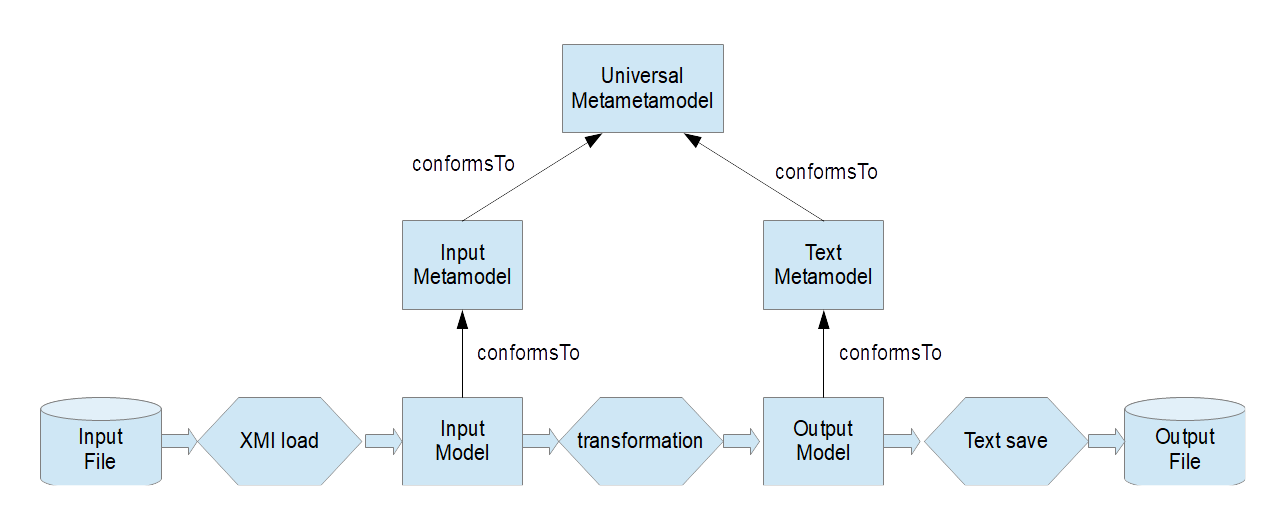
\includegraphics[width=4.9in]{TextM2M.png}
	\end{center}
	\caption{Use of M2M for M2T}
	\label{fig:TextM2M}
\end{figure}

The main challenge is to design a suitable Text metamodel.

\subsection{Text Structure}\label{Text Structure}

Language parsers such as lex and yacc \cite{DragonBook} and their many successors discover the structure of source text by successively aggregating to more powerful concepts:

\begin{itemize}
	\item 8 bit bytes in a source file/stream
	\item Multi-byte characters corresponding to Unicode `letters'
	\item Multi-character tokens corresponding to `words'
	\item Multi-token rules/productions corresponding to `clauses' and `sentences'
\end{itemize}

This conversion sequence is very successful for Text-to-Model conversion but the rules/productions are not appropriate for Model-to-Text conversion since the details of the whitespace formatting are typically discarded once the tokens have been identified. For Model-to-Text purposes, some form of pretty printing is necessary to make the result acceptable to a human reader. We would also like to avoid the language-specific limitations of a typical Text-to-Model grammar.

Traditional M2T tools just concatenate Character Sequences and so we might consider that their \verb$text$ metamodel is just a Sequence of Character. Reifying such a metamodel for M2M usage is easy but the need to assign each character as a distinct model element is pretty unacceptable. Perhaps in QVTo:

\begin{verbatim}
...                                -- 'The name is'
characters += object text::Character { value := ' '; };
characters += object text::Character { value := '"'; };
forEach (c : self.name.characters()) {
    characters += object text::Character { value := c; };
}
characters += object text::Character { value := '"'; };
\end{verbatim}

We should therefore look to some form of multi-Character model.

A significant challenge for practical M2T tools is providing satisfactory indentation and inter-element separation for hierarchical and iterated text structures. The challenge arises because indentation is used within string templates both to indent the output text and to make the control expressions readable. 

For Acceleo, the conflict between template and control characters can require empirical iteration to get a satisfactory result. The documentation recommends use of a separate pretty formatting pass if non-trivial formatting is needed.

The Xtend UI uses a grey background to distinguish template characters. This is helpful but not always perfect since the grey background is omitted from new-line characters. Empirical programming cannot always solve the problem.

\subsection{Text Metamodel}\label{Text Metamodel}

With a Text metamodel, we can separate the concerns. 

\begin{itemize}
	\item The M2M transformation language statements provide a readable exposition.
	\item The Text Model declarations control pretty printing.
\end{itemize}

\begin{figure}
	\begin{center}
		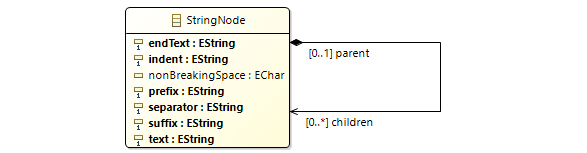
\includegraphics[width=4.9in]{TextModel.png}
	\end{center}
	\caption{Metamodel for Text}
	\label{fig:TextModel}
\end{figure}

The Text model shown in Figure~\ref{fig:TextModel} compromises a tree of StringNode elements organized by \verb$parent$/ordered-\verb$children$ relationships. The additional attributes provide declarations to control the pretty printing performed by the Text Saver.

\subsection{Text Saver}\label{Text Saver}

The result text is formed as the concatenation of a depth-first traversal of the value of the \verb$text$ property of each StringNode.

The detailed formatting of groups of children is facilitated by a \verb$prefix$ before the first, a \verb$separator$ between each child and a \verb$suffix$ after the last child. Additionally an \verb$endText$ may follow the children even if there are no children.

The \verb$indent$ specifies an indentation increment for this node. The cumulative indentation of a node and its parents starts every non-empty line.

An M2M transforms to create the StringNode tree comprising the important text segments and formatting declarations that influence the final serialization. No characters are provided that are not directed by the StringNode.%; it is therefore possible, if desired, to create a text output that is completely free of any new-lines. 

The Text Saver is implemented by a custom EMF TextResource that replaces the conventional XML serialization by the pretty printed text resulting from the depth first tree traversal and formatting declarations.

A corresponding Text Loader is also implemented, mainly for test purposes. The serialization during a Text Save is not fully reversible and so the corresponding replacement functionality when loading is limited to identifying whitespace indentation hierarchies and punctuation separators for matching indentations. Any serious Text-to-Model application probably needs a more powerful approach such as an Xtext parser \cite{Eclipse-Xtext}.

\section{Evaluation}\label{Evaluation}

The Text Model has been used in conjunction with Eclipse QVTo to generate C, H, Lex (Flex) and Y (Bison) files from an Ecore file for an auto-generated XMI loader.

No changes were required to Eclipse QVTo and only a couple of minor bug reports were raised. Problems were easily circumvented. Overall there seemed to be fewer problems than when using Acceleo or Xtend. All approaches share the pleasant characteristic of M2T development that problems are clearly visualized in the textual output. Additional debug output can provide helpful insights. Development time was focussed on the correct content of the Flex and Bison declarations to be generated rather than struggling with their formatting.

Execution of the M2M for text is fast. The 2000 lines of the four XMI loader files are generated in less than a second.

\subsection{Example}\label{Example}

The utility of this approach can be assessed by examining a very simple example that is artificially elaborated to demonstrate important facilities. The target output is the textile snippet shown in Figure~\ref{fig:TextileExample}. The snippet comprises a heading, a blank line then a list of separated formatted elements. 

\begin{figure}
	\begin{center}
		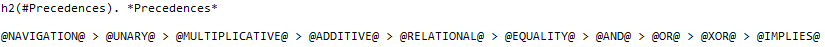
\includegraphics[width=4.9in]{TextileExample.png}
	\end{center}
	\caption{Target Textile Output}
	\label{fig:TextileExample}
\end{figure}

The Acceleo solution in Figure~\ref{fig:AcceleoExample} formats the heading and blank line as literal text at the start of emitPrecedences2. The \verb|[for...]...[/for]| construct supports the formatting of p.name using a \verb|[.../]| escape to access the name. The additional separator argument defines the inter-text separation.

The redundant emitPrecedences1 demonstrates that declarations occur as escapes within the surrounding text literal and the need to re-escape in order to make a nested call. 

\begin{figure}
	\begin{center}
		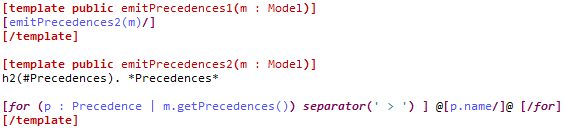
\includegraphics[width=4.9in]{AcceleoExample.png}
	\end{center}
	\caption{Acceleo solution to example}
	\label{fig:AcceleoExample}
\end{figure}

The Xtend solution in Figure~\ref{fig:XtendExample} is very similar except for the guillemet rather than square bracket escapes.

The redundant emitPreferences1 demonstrates that declarations occur as functions within an outer control flow allowing a direct call to a nested function. The inner emitPrecedences2 uses the \verb|'''...'''| backward escape from the outer control to the inner text template formatting. This allows the inner template to be indented for readability.

\begin{figure}
	\begin{center}
		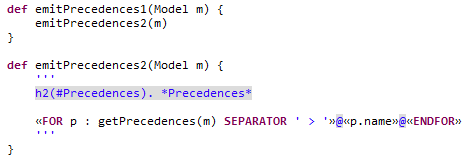
\includegraphics[width=4.5in]{XtendExample.png}
	\end{center}
	\caption{Xtend solution to example}
	\label{fig:XtendExample}
\end{figure}

Finally the new QVTo and Text Model solution is shown in Figure~\ref{fig:QVToExample} is a little more verbose (or a little more modular). The inner formatting is factored out as emitPrecedence3 that constructs a StringNode comprising just the formatted precedence element. Since there is no string template capability, the self.name expression needs no elaboration, but the text needs quoting and concatenation. 

\begin{figure}
	\begin{center}
		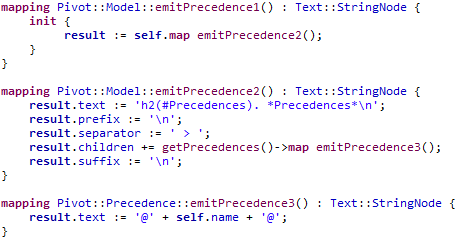
\includegraphics[width=4.0in]{QVToExample.png}
	\end{center}
	\caption{QVTo and Text solution to example}
	\label{fig:QVToExample}
\end{figure}

emitPrecedences2 provides the heading as its text, and iterates emitPrecedences3 to define the children. The separator and children StringNode elements provide very similar capability to the for construct of Acceleo or Xtend. %Use of the prefix and suffix elements to provide the new-lines gives a perhaps more accurate result for the case of no elements.

The redundant emitPrecedences1 demonstrates use of the init section to bypass creation of a nested StringNode. The intermediate Text model instances created by QVTo are shown in Figure~\ref{fig:ExampleInstances}.

\begin{figure}
	\begin{center}
		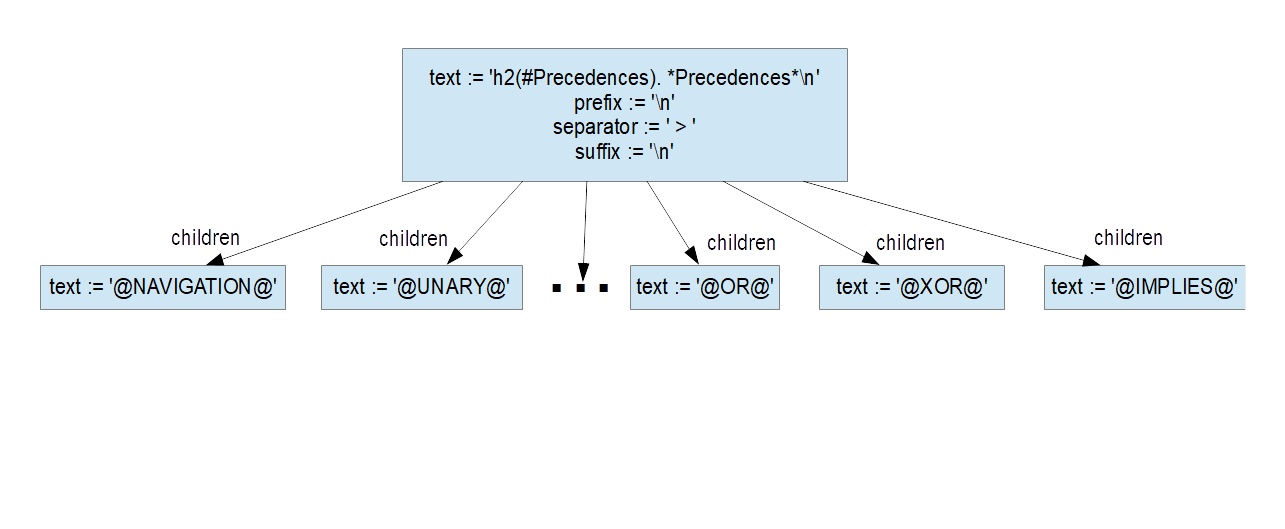
\includegraphics[width=4.9in]{ExampleInstances.png}
	\end{center}
	\caption{StringNode instances for the example}
	\label{fig:ExampleInstances}
\end{figure}

\subsection{MOFM2T}\label{MOFM2T}

The OMG issued the MOF Model to Text Transformation Language Request For Proposal (MOFM2T RFP) in April 2007 as a follow on to the MOF 2.0 Query / Views / Transformations RFP (QVT RFP) which addressed only Model-to-Model transformation. The MOFM2T RFP \cite{MOFM2T-RFP} is very clear in its intent:

\begin{quote}
This RFP calls for a language and semantics for transforming models into text.
The goal is not to create yet another language, but to use or extend existing
OMG language(s). Justification must be provided for creating yet another
language.
\end{quote}

The final MOFM2T submission \cite{MOFM2T-SUB} re-uses the MOF metamodel, OCL expressions
and QVT query syntax. However the orthodoxy of the traditional text templates already in use by the submitters' candidates prevailed. The submission fails to re-use any of the transformation facilities of QVT. It is hard to claim that MOFM2T is not `yet another language'. No justification is provided.

In contrast, in this paper we re-use QVTo (or QVTr or ATL or ...) unchanged to support M2T. This was possible with just one day of development for the one-class metamodel and its associated support.

It might seem that a fully declarative transformation language such as QVTr for M2T could result in the output paragraphs appearing in unpredictable orders? But no, if all collections are ordered, a declarative transformation result should also be ordered; only unordered collections may yield shuffled results.

\section{Future Work}\label{Future Work}

The \verb$http://www.eclipse.org/qvt/2018/TextModel$ metamodel and its support was made available in June 2018 as part of the Eclipse Photon release once the Eclipse QVTd support is also installed. It may be bundled with ATL and/or QVTo in future releases.

The current support is usable. The text model is powerful, but could be extended. More significant is the opportunity for syntax sugar to make that power more accessible.

\subsection{splice iterator}

The inelegance of the splicing at the end of Section~\ref{Text Facilities} may be mitigated by adding a splice() iterator to the OCL Standard Library for ordered collections of toString()-able elements could support:

\begin{verbatim}
'{ '+ somePs->splice(p; separator=',' | '"'+ p.name +'"') +' }'
\end{verbatim}

\subsection{Line Wrapping}\label{Line Wrapping}

Line wrapping is not conventionally available for M2T. The separation of information and rendering concerns enables the Text Model saver to respect a prevailing indentation and line-breaking policy and wrap lines accordingly. Figure~\ref{fig:TextModel}  shows a \verb$nonBreakingSpace$ property that is intended to provide a facility to control automatic wrapping of too-long lines. Long lines are first broken at spaces or tabs, then non-breaking space characters are replaced by space characters.

\subsection{Declarative Pretty Printing}\label{Declarative Pretty Printing}

Tools such as Xtext have demonstrated how the addition of model assignment annotations to an EBNF grammar can synthesize a useful parser/editor rather than just a partial parser. No equivalent extension is available to add pretty-printing annotations, rather Xtext supports manual programming of an independent declarative class. TCS \cite{TCS} has demonstrated that the required line-wrap/space-before/... declarations can be added to an annotated EBNF grammar. The serializer can then be autogenerated as an M2M text transformation. A friendly editor could offer show-assignment-annotations, and show-formatting-annotations options to avoid redundant clutter.

\subsection{String Templates}\label{String Templates}

In the introduction we identified a need to facilitate text synthesis, possibly using a syntax similar to Xtext's triple quote String Template with embedded guillemeted OCL expressions.
The evaluation in Section~\ref{Evaluation} observed that String Templates are not essential, although they may be useful, particularly for output comprising mostly boilerplate.

A string template expression could be added to OCL, in much the same way as it has been to Xtend, 
but learning from Xtend, Acceleo and MOFM2T four escape tokens are needed for the start and end of  a forward or backward escape. Acceleo has only 2, Xtend and MOFM2T just 3 which inhibits arbitrary nesting. Again learning from Xtend, guillemets are very readable and so we might look to use.

\begin{verbatim}
  «ocl-expression»        forwards escape within literal text
  «'string-template'»     backwards escape - an ocl-expression
\end{verbatim}

(An OCL expression starting or ending with a ' can be disambiguated with a space)

These escapes enable the core of our evaluation example from Section~\ref{Evaluation} to nest an ocl-expression within a string-template within an ocl-expression within a string-template within a QVTo statement.

\begin{verbatim}
map Pivot::ModelemitPrecedences2() : Text::StringNode {
    «'
    h2(#Precedences). *Precedences*
	
    «getPrecedences(m)->splice(separator = ', ' | «'@«name»@'»)»
    '»
}
\end{verbatim}

An OCL evaluation of string-templates should compute the appropriate string result. An M2M compilation may recognize that string-templates and splice() are syntax sugar for Text Model capabilities.

%\subsection{Syntax Sugar}\label{Syntax Sugar}

%Construction of a StringNode as a direct consequence of an Eclipse QVTo mapping benefits from the helpful QVTo mapping syntax. Construction of additional StringNode elements requires a verbose \verb$object Text::StringNode { .... }$ wrapper around the nested context. This verbosity can be mitigated by a helper function. A backward escape would be better.

\subsection{Incremental and Parallel M2T}\label{Incremental M2T}

Incremental or parallel execution is difficult in an M2M with imperative characteristics such as QVTo, but very practical in a purely declarative language such as QVTr. Therefore if QVTr is used as the M2M, an incremental execution can mark dirty StringNode elements in the tree that can then be selectively reserialized. Unfortunately incremental QVTr execution is not yet available. A parallel execution can distribute parts of the StringNode tree to multiple proocessors and bring the results together at the end.

\section{Related Work}\label{Related Work}

Defining a really simple text model to allow an M2M to be used for an M2T seems like a rather obvious idea. However string template orthodoxy is so entrenched that this simple tree model seems to have been overlooked. Consequently many tools and researchers use naive Strings and then struggle to recover lost structure.

Ogunyomi \cite{Signatures} introduces user-defined signatures to facilitate identifying text segments that need updating. These should be available automatically as a consequence of dependency analysis in a declarative M2M. 

Figure~\ref{fig:M2MM2TFeatureModel} shows a Feature Model for our use of M2M for M2T in the style proposed by Rose \cite{Feature Model}. 

\begin{figure}
	\begin{center}
		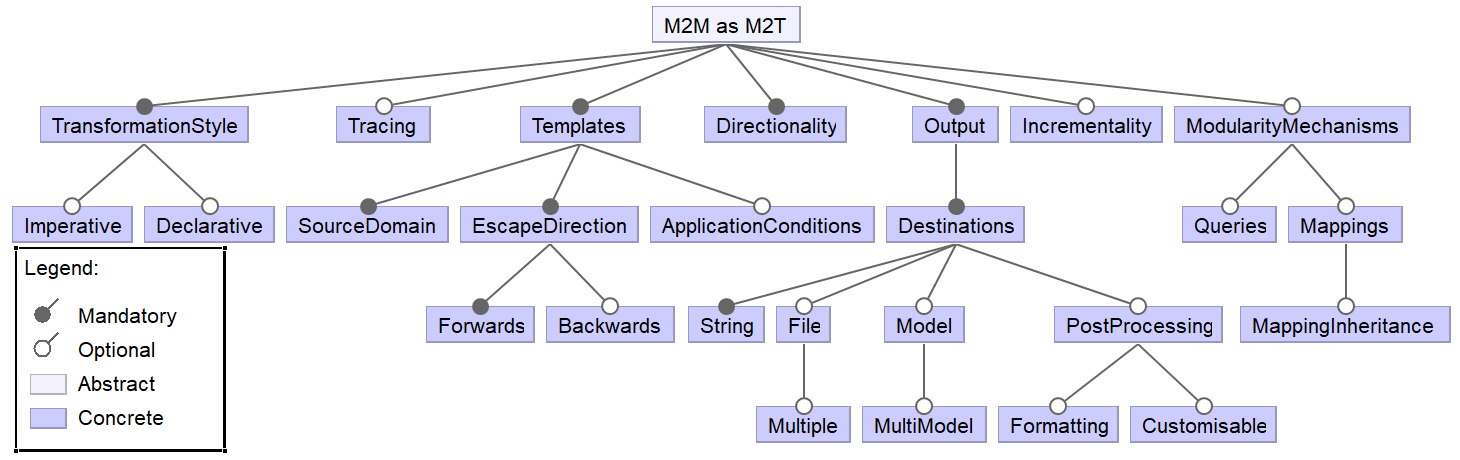
\includegraphics[width=4.9in]{M2MM2TFeatureModel.png}
	\end{center}
	\caption{Feature Model for M2M used for M2T}
	\label{fig:M2MM2TFeatureModel}
\end{figure}

This highlights that the mandatory forwards escaping is missing; we have proposed an OCL extension to remedy this. In other respects, the M2M facilities provide good feature coverage and additional features regarding model output. The external text model provides for extensibility.

\section{Conclusions}\label{Conclusions}

We have introduced a very simple one-class metamodel that models text as a tree of attributed character sequences.

We have shown that this metamodel separates the content and pretty printing concerns and enables any M2M to be used without modification as an M2T.

We have demonstrated the usability of this approach by using Eclipse QVTo to generate c, h, lex and y files from an Ecore metamodel.

We have outlined minor extensions to OCL to improve OCL-based M2M usability for M2T.

We can therefore argue that this simple approach to M2T is more compliant with the OMG MOFM2T RFP than the eventual MOFM2T standard.


% ---- Bibliography ----
%
\begin{thebibliography}{}
%
\bibitem{DragonBook}
Aho, A., Sethi, R., Ullman, J.: Compilers, Principles, Techniques and Tools, Addison Wesley, 1986

\bibitem{SAXparser}
Brownell, D.: SAX2, 'Reilly, 2002, ISBN 0-596-00237-8.

\bibitem{TechnologySpace}
Ivanov, I., B\'ezivin, J., Aksit, M.: Technological Spaces: An Initial Appraisal. 1-6.  (2002). 

\bibitem{TCS}
Jouault, F.,  B\'ezivin, J.,  Kurtev. I.: TCS: A DSL for the specification of textual concrete syntaxes in model engineering. Model-Driven Engineering Languages and Systems: 17th International Conference, MODELS 2014, , September 28 – October 3, 2014, Valencia, Spain.
\url{https://research.utwente.nl/en/publications/tcsa-dsl-for-the-specification-of-textual-concrete-syntaxes-in-mo}

\bibitem{Signatures}
Ogunyomi, B., Rose, L., Kolovos, D.: User-defined Signatures for Source Incremental Model-to-text Transformation. 5th International Conference, GPCE 2006, Portland, Oregon, USA, October 22-26, 2006.
\url{http://ceur-ws.org/Vol-1331/p4.pdf}

\bibitem{Feature Model}
Rose, L., Matragkas, N., Kolovos, D.,  Paige, R.: A feature model for model-to-text transformation languages. In Modeling in Software Engineering (MISE), 2012 ICSE Workshop on (pp. 57-63). IEEE. DOI: 10.1109/MISE.2012.6226015

\bibitem{Bug396543}
Siljamaki, T.: Additional M2T capability in QVTO. Eclipse QVTo project Bugzilla 396543. December, 2012.
\url{https://bugs.eclipse.org/396543}

\bibitem{MOFM2T-RFP}
MOF Model to Text Transformation Language Request For Proposal. OMG Document: ad/04-04-07, April 2004.
\url{https://www.omg.org/cgi-bin/doc?ad/04-04-07.pdf}

\bibitem{MOFM2T-SUB}
Revised submission for MOF Model to Text Transformation Language RFP. OMG Document: ad/06-09-03. September 2006.
\url{https://www.omg.org/cgi-bin/doc?ad/06-09-03.pdf}

\bibitem{MOFM2T-1.0}
MOF Model to Text Transformation Language, v1.0, OMG Document Number: formal/2008-01-16, Object Management Group (2008),  \url{http://www.omg.org/spec/MOFM2T/1.0}

\bibitem{OCL-2.4}
Object Constraint Language. Version 2.4., OMG Document Number: formal/2014-02-03, Object Management Group (2009),  \url{http://www.omg.org/spec/OCL/2.4}

\bibitem{QVT-1.3}
OMG. Meta Object Facility (MOF) 2.0 Query/View/Transformation Specification, Version 1.3.
OMG Document Number: ptc/16-06-03, June 2016.

\bibitem{Eclipse-Acceleo}
Eclipse Acceleo Project.\\
\url{https://projects.eclipse.org/projects/modeling.m2t.acceleo}

\bibitem{Eclipse-ATL}
Eclipse ATL Project.\\
\url{https://projects.eclipse.org/projects/modeling.mmt.atl}

\bibitem{Eclipse-QVTd}
Eclipse QVT Declarative Project.\\
\url{https://projects.eclipse.org/projects/modeling.mmt.qvtd}

\bibitem{Eclipse-QVTo}
Eclipse QVT Operational Mappings Project.\\
\url{https://projects.eclipse.org/projects/modeling.mmt.qvto}

\bibitem{Eclipse-Xtext}
Eclipse Xtext Project.\\
\url{https://projects.eclipse.org/projects/modeling.tmf.xtext}

\end{thebibliography}
\end{document}
